\subsection{connection setup code: client (C)}
\begin{frame}[fragile,label=connSetupClientAddrInfo]{connection setup: client, using addrinfo}
\begin{lstlisting}[
    language=C++,style=smaller,
    moredelim={**[is][\btHL<2|handout:2>]{@2}{2@}},
    moredelim={**[is][\btHL<3|handout:3>]{@3}{3@}},
    moredelim={**[is][\btHL<4|handout:4>]{@4}{4@}},
    moredelim={**[is][\btHL<5|handout:5>]{@5}{5@}},
    moredelim={**[is][\btHL<6|handout:6>]{@6}{6@}},
]
int sock_fd; 
@2struct addrinfo2@ *server = /* code on next slide */;

sock_fd = socket(
    @3server->ai_family3@,  
     // ai_family = AF_INET (IPv4) or AF_INET6 (IPv6) or ...
    @3server->ai_socktype3@,
     // ai_socktype = SOCK_STREAM (bytes) or ...
    @3server->ai_prototcol3@
     // ai_protocol = IPPROTO_TCP or ...
);
if (sock_fd < 0) { /* handle error */ }
if (connect(sock_fd, server->@4ai_addr4@, server->@4ai_addrlen4@) < 0) {
    /* handle error */
}
@5freeaddrinfo(server);5@
DoClientStuff(sock_fd); /* read and write from sock_fd */
close(sock_fd);
\end{lstlisting}
\begin{tikzpicture}[overlay,remember picture]
\tikzset{
    box/.style={draw=red, ultra thick,fill=white,at={([yshift=-2cm]current page.north)},anchor=north,align=left},
    box low/.style={draw=red, ultra thick,fill=white,at={([yshift=-5cm]current page.north)},anchor=north,align=left},
}
\begin{visibleenv}<2>
\node[box low] {
    addrinfo contains all information needed to setup socket \\
    set by \texttt{getaddrinfo} function (next slide) \\
    handles IPv4 and IPv6 \\
    handles DNS names, service names
};
\end{visibleenv}
\begin{visibleenv}<4>
\node[box] {
    ai\_addr points to struct representing address \\
    type of struct depends whether IPv6 or IPv4
};
\end{visibleenv}
\begin{visibleenv}<5>
\node[box] {
    since addrinfo contains pointers to dynamically allocated memory, \\
    call this function to free everything
};
\end{visibleenv}
\end{tikzpicture}
\end{frame}

\begin{frame}[fragile,label=serverLookupClient]{connection setup: lookup address}
\begin{lstlisting}[
    language=C++,style=smaller,
    moredelim={**[is][\btHL<2|handout:2>]{@2}{2@}},
    moredelim={**[is][\btHL<3|handout:3>]{@3}{3@}},
    moredelim={**[is][\btHL<4|handout:4>]{@4}{4@}},
    moredelim={**[is][\btHL<5|handout:5>]{@5}{5@}},
    moredelim={**[is][\btHL<6|handout:6>]{@6}{6@}},
]
/* example hostname, portname = "www.cs.virginia.edu", "443" */
const char *hostname; const char *portname;
...
struct addrinfo *server;
struct addrinfo hints;
int rv;
memset(&hints, 0, sizeof(hints));
@3hints.ai_family = AF_UNSPEC3@; /* for IPv4 OR IPv6 */
// hints.ai_family = AF_INET4; /* for IPv4 only */

hints.ai_socktype = SOCK_STREAM; /* byte-oriented --- TCP */
rv = getaddrinfo(hostname, portname, &hints, @2&server2@);
if (rv != 0) { /* handle error */ }

/* eventually freeaddrinfo(result) */
\end{lstlisting}
\begin{tikzpicture}[overlay,remember picture]
\tikzset{
    box/.style={draw=red, ultra thick,fill=white,at={([yshift=-2cm]current page.north)},anchor=north,align=left},
    box low/.style={draw=red, ultra thick,fill=white,at={([yshift=-5cm]current page.north)},anchor=north,align=left},
}
\begin{visibleenv}<2>
\node[box low] {
    NB: pass pointer \textit{to pointer} to addrinfo to fill in
};
\end{visibleenv}
\begin{visibleenv}<3>
\node[box] {
    AF\_UNSPEC: choose between IPv4 and IPv6 for me \\
    AF\_INET, AF\_INET6: choose IPv4 or IPV6 respectively
};
\end{visibleenv}
\end{tikzpicture}
\end{frame}
 

\subsection{connection setup code: server (C)}
\begin{frame}[fragile,label=connSetupServerLookup]{connection setup: server, address setup}
\begin{lstlisting}[
    language=C++,style=smaller,
    moredelim={**[is][\btHL<2|handout:2>]{@2}{2@}},
    moredelim={**[is][\btHL<3|handout:3>]{@3}{3@}},
    moredelim={**[is][\btHL<4|handout:4>]{@4}{4@}},
    moredelim={**[is][\btHL<5|handout:5>]{@5}{5@}},
    moredelim={**[is][\btHL<6|handout:6>]{@6}{6@}},
]
/* example (hostname, portname) = ("127.0.0.1", "443") */
const char *@2hostname2@; const char *@3portname3@;
...
struct addrinfo *server;
struct addrinfo hints;
int rv;

memset(&hints, 0, sizeof(hints));
hints.ai_family = AF_INET; /* for IPv4 */
/* or: */ hints.ai_family = AF_INET6; /* for IPv6 */
/* or: */ hints.ai_family = AF_UNSPEC; /* I don't care */
@4hints.ai_flags = AI_PASSIVE4@;

rv = getaddrinfo(hostname, portname, &hints, &server);
if (rv != 0) { /* handle error */ }
\end{lstlisting}
\begin{tikzpicture}[overlay,remember picture]
\tikzset{
    box/.style={draw=red, ultra thick,fill=white,at={([yshift=-2cm]current page.north)},anchor=north,align=left},
    box low/.style={draw=red, ultra thick,fill=white,at={([yshift=-6cm]current page.north)},anchor=north,align=left},
}
\begin{visibleenv}<2>
\node[box low] {
    \texttt{hostname} could also be NULL \\
    means ``use all possible addresses'' \\
    only makes sense for servers
};
\end{visibleenv}
\begin{visibleenv}<3>
\node[box low] {
    \texttt{portname} could also be NULL \\
    means ``choose a port number for me'' \\
    only makes sense for servers
};
\end{visibleenv}
\begin{visibleenv}<4>
\node[box] {
    AI\_PASSIVE: ``I'm going to use bind''
};
\end{visibleenv}
\end{tikzpicture}
\end{frame}


\begin{frame}[fragile,label=connSetupServerAddrinfo]{connection setup: server, addrinfo}
\begin{lstlisting}[
    language=C++,style=smaller,
    moredelim={**[is][\btHL<2|handout:2>]{@2}{2@}},
    moredelim={**[is][\btHL<3|handout:3>]{@3}{3@}},
    moredelim={**[is][\btHL<4|handout:4>]{@4}{4@}},
    moredelim={**[is][\btHL<5|handout:5>]{@5}{5@}},
    moredelim={**[is][\btHL<6|handout:6>]{@6}{6@}},
]
struct addrinfo *server;
... getaddrinfo(...) ...

int server_socket_fd = socket(
    server->ai_family,
    server->ai_sockttype,
    server->ai_protocol
);

if (bind(server_socket_fd, ai->ai_addr, ai->ai_addr_len)) < 0) {
    /* handle error */
}
listen(server_socket_fd, MAX_NUM_WAITING);
...
int socket_fd = accept(server_socket_fd, NULL);
\end{lstlisting}
\end{frame}

 

\subsection{more manual setup in C}
\subsubsection{client}
\begin{frame}[fragile,label=connSetupClientManual]{connection setup: client --- manual addresses}
\begin{lstlisting}[
    language=C++,style=smaller,
    moredelim={**[is][\btHL<1|handout:1>]{@1}{1@}},
    moredelim={**[is][\btHL<2|handout:2>]{@2}{2@}},
    moredelim={**[is][\btHL<3|handout:3>]{@3}{3@}},
    moredelim={**[is][\btHL<4|handout:4>]{@4}{4@}},
    moredelim={**[is][\btHL<5|handout:5>]{@5}{5@}},
    moredelim={**[is][\btHL<6|handout:6>]{@6}{6@}},
]
int sock_fd;

server = /* code on later slide */;
sock_fd = @1socket1@(
    @2AF_INET2@, /* IPv4 */
    @2SOCK_STREAM2@, /* byte-oriented */
    @2IPPROTO_TCP2@
);
if (sock_fd < 0) { /* handle error */ }

@4struct sockaddr_in addr4@;
addr.sin_family = AF_INET;
addr.sin_addr.s_addr = @3htonl3@(2156872459); /* 128.143.67.11 */
addr.sin_port = @3htons3@(80); /* port 80 */
if (@1connect1@(sock_fd, (struct sockaddr*) &addr, sizeof(addr)) {
    /* handle error */
}
DoClientStuff(sock_fd); /* read and write from sock_fd */
close(sock_fd);
\end{lstlisting}
\begin{tikzpicture}[overlay,remember picture]
\tikzset{
    box/.style={draw=red, ultra thick,fill=white,at={([yshift=-2cm]current page.north)},anchor=north,align=left},
    box low/.style={draw=red, ultra thick,fill=white,at={([yshift=-5cm]current page.north)},anchor=north,align=left},
}
\begin{visibleenv}<2>
\node[box low] {
    specify IPv4 instead of IPv6 or local-only sockets \\
    specify TCP (byte-oriented) instead of UDP (`datagram' oriented)
};
\end{visibleenv}
\begin{visibleenv}<3>
\node[box] {
    htonl/s = host-to-network long/short \\
    network byte order = big endian
};
\end{visibleenv}
\begin{visibleenv}<4>
\node[box] {
    struct representing IPv4 address + port number \\
    declared in \lstinline|<netinet/in.h>| \\
    see \texttt{man 7 ip} on Linux for docs
};
\end{visibleenv}
\end{tikzpicture}
\end{frame}
 
\subsubsection{server}
\begin{frame}[fragile,label=connSetupServer]{connection setup: server, manual}
\begin{lstlisting}[
    language=C++,style=smaller,
    moredelim={**[is][\btHL<2|handout:2>]{@2}{2@}},
    moredelim={**[is][\btHL<3|handout:3>]{@3}{3@}},
    moredelim={**[is][\btHL<4|handout:4>]{@4}{4@}},
    moredelim={**[is][\btHL<5|handout:5>]{@5}{5@}},
    moredelim={**[is][\btHL<6|handout:6>]{@6}{6@}},
]
int server_socket_fd = socket(AF_INET, SOCK_STREAM, IPPROTO_TCP);
struct sockaddr_in addr;
addr.sin_family = AF_INET;
addr.sin_addr.s_addr = @2INADDR_ANY2@; /* "any address I can use" */
    @3/* or: addr.s_addr.in_addr = INADDR_LOOPBACK (127.0.0.1) */3@
    /* or: addr.s_addr.in_addr = htonl(...); */
addr.sin_port = @4htons(9999)4@; /* port number 9999 */

if (bind(server_socket_fd, &addr, sizeof(addr)) < 0) {
    /* handle error */
}
listen(server_socket_fd, @4MAX_NUM_WAITING4@);
...
int socket_fd = accept(server_socket_fd, NULL);
\end{lstlisting}
\begin{tikzpicture}[overlay,remember picture]
\tikzset{
    box/.style={draw=red, ultra thick,fill=white,at={([yshift=-2cm]current page.north)},anchor=north,align=left},
    box low/.style={draw=red, ultra thick,fill=white,at={([yshift=-6cm]current page.north)},anchor=north,align=left},
}
\begin{visibleenv}<2>
\node[box low] {
    INADDR\_ANY: accept connections for any address I can! \\
    alternative: specify specific address
};
\end{visibleenv}
\begin{visibleenv}<3>
\node[box low] {
    bind to 127.0.0.1? only accept connections \myemph{from same machine} \\
    what we recommend for FTP server assignment
};
\end{visibleenv}
\begin{visibleenv}<4>
\node[box low] {
    choose the number of unaccepted connections
};
\end{visibleenv}
\end{tikzpicture}
\end{frame}
 

\subsection{gethostbyname}
\begin{frame}[fragile,label=serverLookupClientOld]{connection setup: old lookup function}
\begin{lstlisting}[language=C++,style=smaller]
/* example hostname, portnum= "www.cs.virginia.edu", 443*/
const char *hostname; int portnum;
...
struct hostent *server_ip;
server_ip = gethostbyname(hostname);

if (server_ip == NULL) { /* handle error */ }

struct sockaddr_in addr;
addr.s_addr = *(struct in_addr*) server_ip->h_addr_list[0];
addr.sin_port = htons(portnum);
sock_fd = socket(AF_INET, SOCK_STREAM, IPPROTO_TCP);
connect(sock_fd, &addr, sizeof(addr));
...
\end{lstlisting}
\end{frame}
 

\subsection{send/recv}


\begin{frame}{aside: send/recv}
    \begin{itemize}
    \item sockets have some alternate read/write-like functions:
        \begin{itemize}
        \item recv, recvfrom, recvmsg
        \item send, sendmsg
        \end{itemize}
    \item have some additional options we won't need in this class
    \end{itemize}
\end{frame}


\subsection{getting addresses from sockets}
\begin{frame}{aside: getting addresses}
\begin{itemize}
\item Python: \texttt{sock.getsockname() == (addr, port)} of local side
\item Python: \texttt{sock.getpeername() == (addr, port)} of remote side
\end{itemize}
\end{frame}


\subsection{basic flow}
\usetikzlibrary{arrows.meta}

\begin{frame}{connected sockets}
    \begin{itemize}
    \item ``connected'' sockets can represent a connection
    \end{itemize}
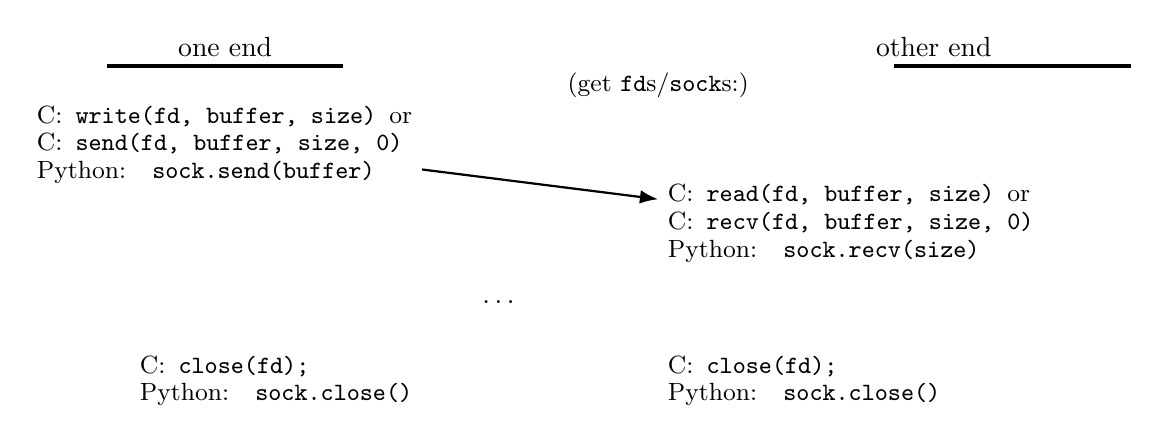
\begin{tikzpicture}
\tikzset{>=Latex}
\node[anchor=south] at (1.5, 0) {one end};
\draw[ultra thick] (0, 0) -- ++(3, 0);
\draw[ultra thick] (10, 0) -- ++(3, 0);
\node[anchor=south] at (10.5, 0) {other end};
\node[font=\small] at (7, -.25) {(get \texttt{fd}s/\texttt{sock}s:)};
\tikzset{
    function/.style={font=\fontsize{9}{10}\tt\selectfont,align=left},
}
\node[function,anchor=east] (write 1) at (4, -1) {
{\normalfont C:} write(fd, buffer, size) \textit{\normalfont or} \\
{\normalfont C:} send(fd, buffer, size, 0) \\
{\normalfont Python:} sock.send(buffer) 
};
\node[function,anchor=west] (read 1) at (7, -2) {
{\normalfont C:} read(fd, buffer, size) \textit{\normalfont or} \\
{\normalfont C:} recv(fd, buffer, size, 0) \\
{\normalfont Python:} sock.recv(size) 
};
\draw[thick,->] (write 1) -- (read 1);
\node at (5, -3) {\ldots};
\node[function,anchor=east] at (4, -4) {
    {\normalfont C:} close(fd); \\
    {\normalfont Python:} sock.close()
};
\node[function,anchor=west] at (7, -4) {
    {\normalfont C:} close(fd); \\
    {\normalfont Python:} sock.close()
};
\end{tikzpicture}
\end{frame}

